\documentclass[]{article}

\usepackage{subcaption}
\usepackage{amssymb,amsmath,amsthm}
\usepackage{svg}
\usepackage{caption, subcaption}
\usepackage[backend=bibtex]{biblatex}  
\usepackage{todonotes}
\usepackage{graphicx}
\usepackage{hyperref}
\usepackage{etoolbox}

\graphicspath{ {./images/} }

\title{Literature Review on Cell tracking across videos from different points of view}
\author{Chrysostomos Chadjiminas 
	\\[0.55cm]{\small Advisor: Dr. Adam Dubis}}


\addbibresource{biblio.bib} 
\AtEndDocument{
	\clearpage
	\printbibliography
}

\begin{document}

\maketitle

\section{Introduction}

In this thesis the main goal is to measure red blood cells velocity as 
they move inside the capillaries of the retina.
A video of the back of the eye is captured using an Adaptive Optics Light Scanning Opthalmoscope that was developed by my supervisor and his team.
From having video of the red blood cell(erythrocyte) movement, one can deduce the velocity of the blood flow, among other characteristics.
To measure the blood flow velocity, the  erythrocytes must be detected across the frames. 
Because the video is captured at a known fixed rate and the field of view is known, the velocity of each red blood cell can be calculated
which could be important for examining whether the blood flow is normal.

% Παράφραση from the Adam Dubis email
The retina is unique because, with development in adaptive optics, it allows for a non-invasive imaging of the vascular plexus inside the retina \cite{tam_noninvasive_2010}.
As the vascular system gets older, or damage is done to it from different diseases such as diabetes, heart disease, chronic inflammatory diseases or other neurological diseases, the arterial blood vessels are not able to dampen the rate of blood flow as they used to.
As a result, the pressure wave tracks down the blood vessel (arteries and veins) and into the capillaries. 
These changes occur before the disease is detected. 
Contrary to the symptoms these diseases show at a later stage, the changes potentially be reversed, effectively preventing the disease from causing more damage.
It is believed that this loss of vessel pulse dampening is responsible the disease effects of diabetes \cite{mizutani_accelerated_diabetes_1996}, dementia \cite{de_la_torre_is_alzheimer_2004}, stroke \cite{ostergaard_role_stroke_2013}, hypertension \cite{wolf_s_quantification_hypertension_1994}, Parkinson's and Multiple Sclerosis \cite{bateman_comparison_multiple_sclerosis_2016}.
The capillaries of the brain could serve as an effective biomarker for the existence of such diseases.
Unfortunately, examining these small vessels and the blood flow in the brain can be hard, expensive or sometimes impossible.
However, the vascular system of the eye and brain are similar to each other and different from everywhere else in the body.
As a result, the imaging of the retinal vasculature could accurate reflect the microvascular changes that happen in the brain \cite{patton_retinal_brain_vasculature_similarity_2005}. ``The eye is the window of the soul'', and more specifically, a window to the brain.

As previously mentioned, our goal is to measure the velocity of the blood cells as captured in videos of the capillaries inside the retina.
Manually detecting the blood cell's in these images and finding the correspondence is slow, cumbersome, and error prone.
Therefore, we want to develop an automated technique to detect and track the blood cells across the video to extract the blood flow velocity.
There are many challenges that must be overcome and a lot of work is done to solve similar problems.

In the next sections we will discuss related work and while also stating how our work could benefit from it.


\section{Literature review}
First we would like to present the method that is used to produce the images and videos shown in Fig \ref{fig:own-retinal-capillaries}.

Before doing that, it's good to briefly introduce Adaptive Optics Laser Opthalmoscope imaging for capturing images of the retina.

\subsection*{Confocal Imaging and Adaptive Optics Scanning Laser Ophthalmoscope (AOSLO)}

In optical confocal imaging, a laser beam of a non harmful wavelength is shone in to the eye. 
The ray is then focused to narrow depth of field and is reflected back to a sensor.
The beam scans the retina in a raster fashion with a fixed rate until the raster image
of the desired size is created.
The scanning beam frequency and the size of the frame affect the frame rate of the 
produced video.
Confocal imaging alone produces distorted and noisy results.
Adaptive optics introduces a deformable mirror to correct distorted wavefronts producing higher fidelity signal.
Such techniques allow microvascular examination imaging of the retina\cite{chui_use_2012}.
AOSLO applies for non-confocal imaging as well but it's out of scope for this report.

\begin{figure}[ht]
	\centering
	\begin{subfigure}[t]{0.49\textwidth}
		\centering
		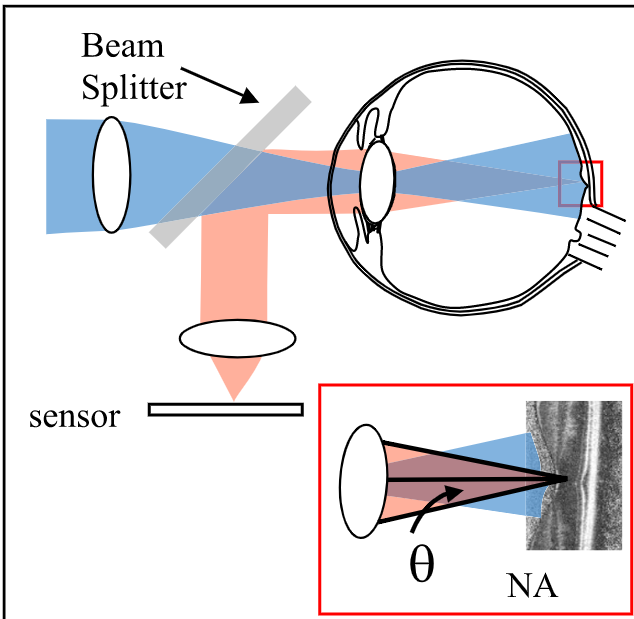
\includegraphics[width=0.65\textwidth]{confocal_imaging_eye.png}
		\caption{}
		\label{fig:confocal-microscopy}
	\end{subfigure}
	\hfil
	\begin{subfigure}[t]{0.49\textwidth}
		\centering
		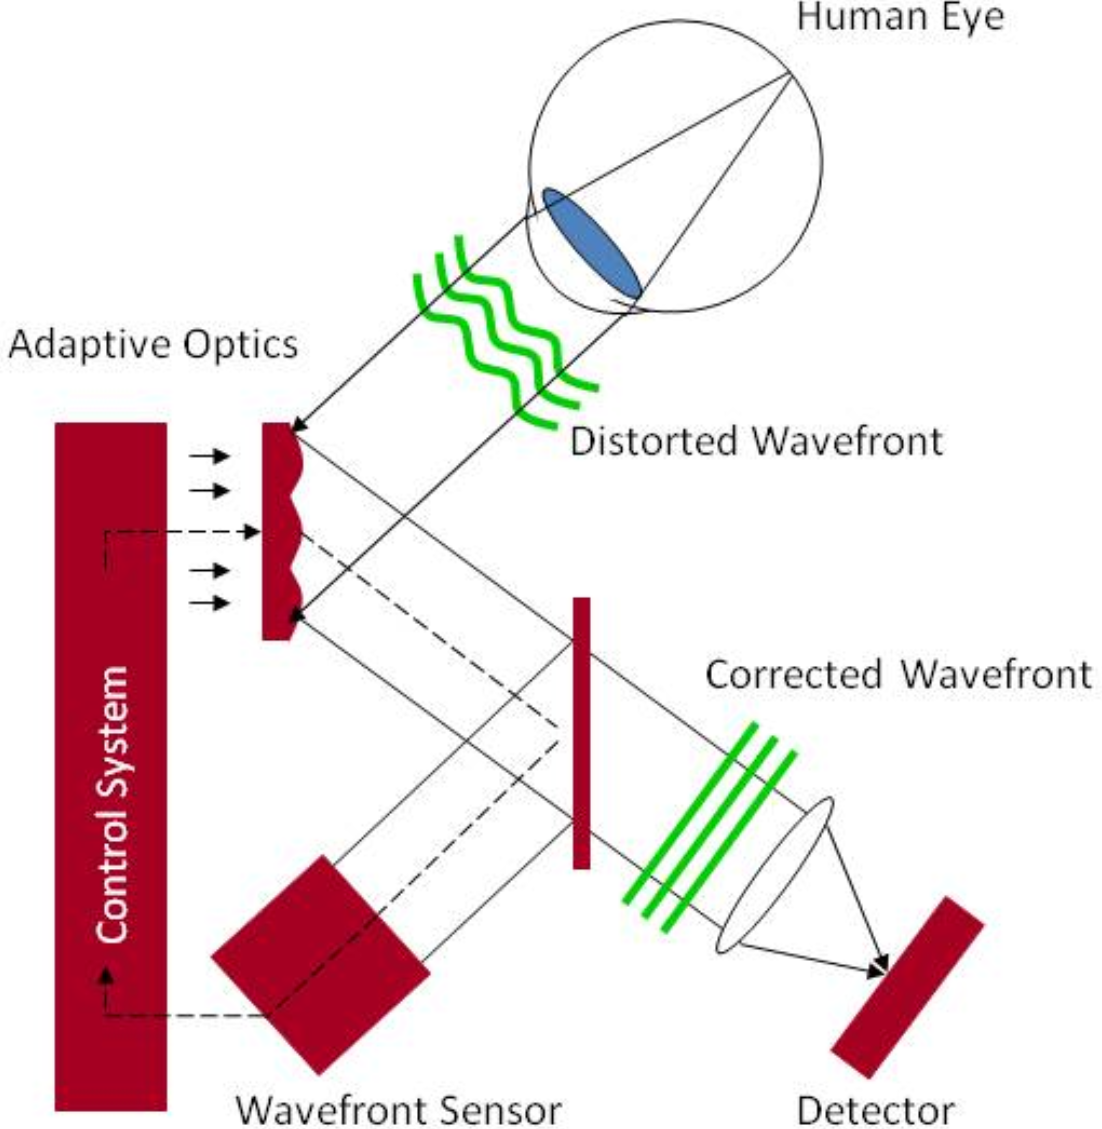
\includegraphics[width=0.75\textwidth]{Adaptive_Imaging.png}
		\caption{}
		\label{fig:adaptic-optics}
	\end{subfigure}
	\caption{\ref{fig:confocal-microscopy} Image from\cite{burns_adaptive_2019}. 
	Conformal microscopy, A laser is shone to the eye and the beam is reflected back to a sensor.\ref{fig:adaptic-optics} Image from\cite{adaptive_image}. Adaptive optics introduces a deform-able mirror to correct distorted wavefront.
	The corrected signal is collected from the detector.
	}
	\label{fig:labep}
\end{figure}

\begin{figure}
	\centering
	\begin{subfigure}[t]{0.45\textwidth}
		\centering
		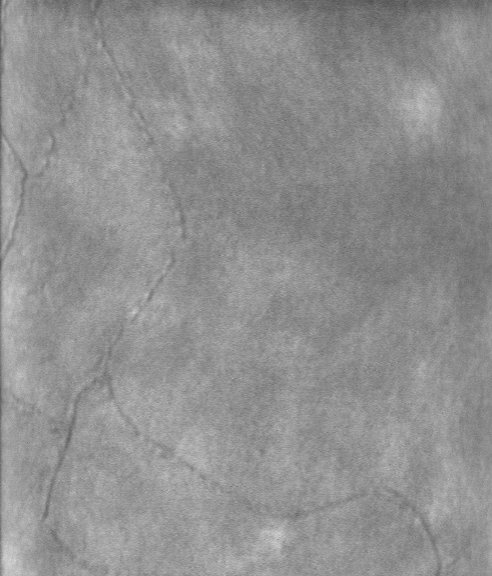
\includegraphics[scale=0.3]{Subject3_Session216_OD_(0,0)_1x1_980_OA790nm_dewarped_first.jpg}
		\caption{An image captured with AOSLO of a retinal capillary.}
		\label{fig:eye-capillary}
	\end{subfigure}
	\hfill
	\centering
	\begin{subfigure}[t]{0.45\textwidth}
		\centering
		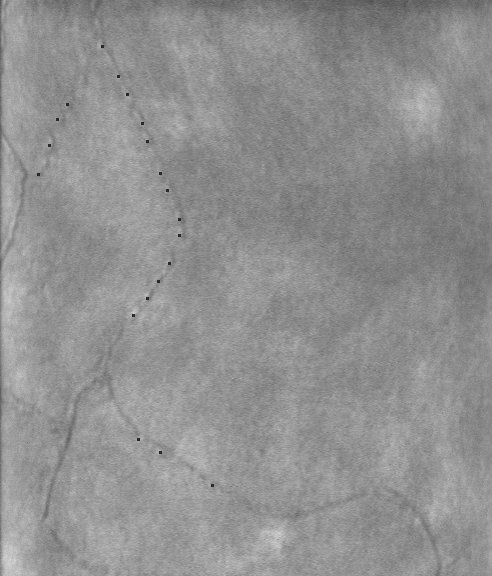
\includegraphics[scale=0.3]{Subject3_Session216_OD_(0,0)_1x1_980_OA790nm_marked_first.jpg}
		\caption{The same image with the blood cells marked}
		\label{fig:eye-capillary-marked}
	\end{subfigure}
	\vfill
	\centering
	\begin{subfigure}[t]{\textwidth}
		\centering
		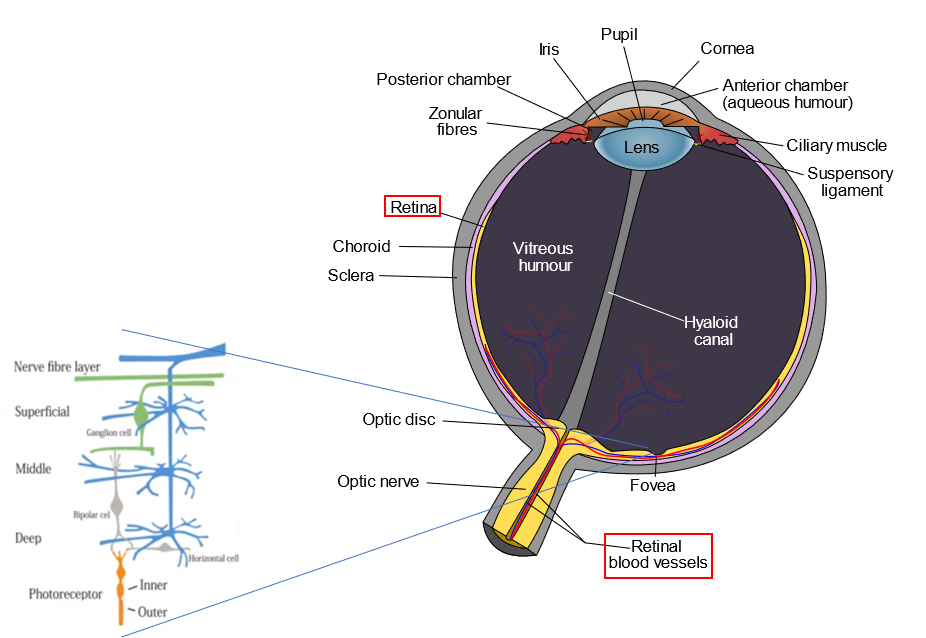
\includegraphics[width=\textwidth]{eye_anatomy.png}
		\caption{A picture of the eye anatomy\cite{eye_anatomy}.}
		\label{fig:eye-anatomy}
	\end{subfigure}
	\caption{\ref{fig:eye-capillary} \ref{fig:eye-capillary-marked} A still frame of a raster image captured using the AOSLO technique described in \cite{castro_rapid_2016}.
		The depth of field captures the red blood cells as they move in the capillaries in middle to deep levels of the retina as seen in \ref{fig:eye-anatomy}.
		The frame is a part of a bigger video found in this media link: \href{https://youtu.be/-7ew5sqOaTo}{(media)}.
	\ref{fig:eye-anatomy} The arteries and veins are fed through the optical nerve.
	In the image on the left\cite{noauthor_varying_nodate} we see that the retina hosts
	small vessels at many levels. }
	\label{fig:own-retinal-capillaries}
\end{figure}

\subsection{Rapid high resolution image with dual-channel scanning technique\cite{castro_rapid_2016}}
Our group build a system based on\cite{castro_rapid_2016}.
The Rapid high resolution image with dual-channel scanning technique uses Adaptive Optics Laser Opthalmoscope (AOSLO) to produce two images of the same area in the retina with a very small time displacement.
Producing a single video of the capillaries with one channel captured at a frame of rate 32fps is not
enough because the time disparity between the two frames is too large and the correspondence of the frames can not be established.
This produces an aliasing effect that is demonstrated in Fig \ref{fig:aliasing-effect}.

\begin{figure}[ht]
	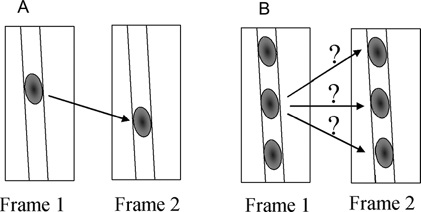
\includegraphics[width=\textwidth]{aliasing-effect.jpg}
	\caption{Image demonstrating aliasing effects from\cite{japee_automated_2005}. =
		 The red blood cells are abundant in the capillaries and they move fast.
	     As seen in B If the frame rate is not fast enough the time difference between the 
     	 between the frames is large so that it's impossible to establish a correspondence 
     	 between the cells in two consecutive frames.}
	\label{fig:aliasing-effect}
\end{figure}

To overcome this problem, the work in\cite{castro_rapid_2016} proposes a new technique where two different slightly different imaging wavelengths are used at the same time.
As a result, two rasters of the same retina area are produced with a very small time disparity making it possible to establish a correspondence.
The two images produces are called channels of the same frame since they correspond to the same retinal area but with a small temporal difference.
The time difference in\cite{castro_rapid_2016} is  4.7 ms while the implementation of our team currently achieves 5.3ms due to differences between our scanners and the device used in the paper.
Another advantage of this technique is that this is a configurable value and may change over time.
For a demonstration of the results please see Fig \ref{fig:corresponding-channels}.

\begin{figure}[ht]
	\centering
	\begin{subfigure}[b]{.4\textwidth}
		\centering
		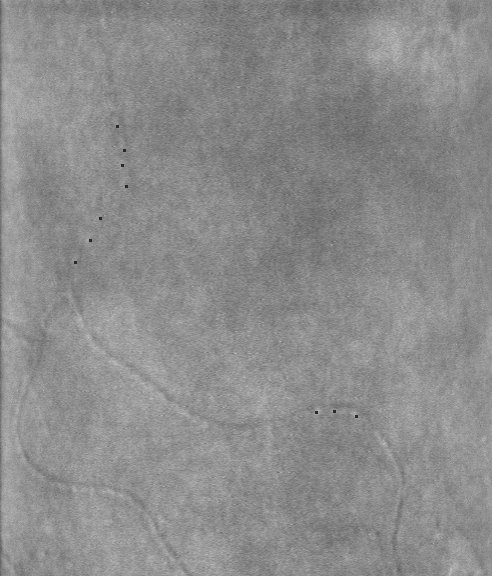
\includegraphics[width=0.75\textwidth, scale=0.75]{Subject3_Session216_OD_(0,0)_1x1_980_OA850nm_marked.jpg}
		\caption{Own image, channel 1 (790nm wavelength)}
		\label{fig:own-channel-a}
	\end{subfigure}
	\hfill
	\centering
	\begin{subfigure}[b]{.4\textwidth}
		\centering
		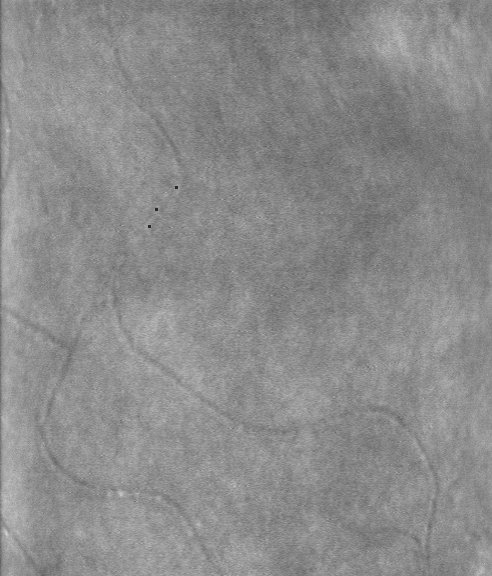
\includegraphics[width=0.75\textwidth, scale=0.75]{Subject3_Session216_OD_(0,0)_1x1_980_OA850nm_marked_corresponding_image.jpg}
		\caption{Own image, channel 2 (850nm wavelength)}
		\label{fig:own-channel-b}
	\end{subfigure}
	\vfill
	\centering
	\begin{subfigure}[t]{.4\textwidth}
		\centering
		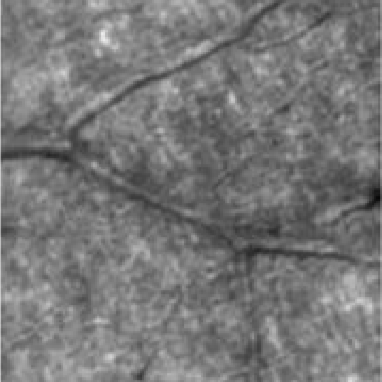
\includegraphics[width=0.75\textwidth, scale=0.75]{de_castro_channel_1.png}
		\caption{Image from \cite{castro_rapid_2016}, channel 1}
		\label{fig:de-castro-channel-a}
	\end{subfigure}
	\hfill
	\centering
	\begin{subfigure}[t]{0.4\textwidth}
		\centering
		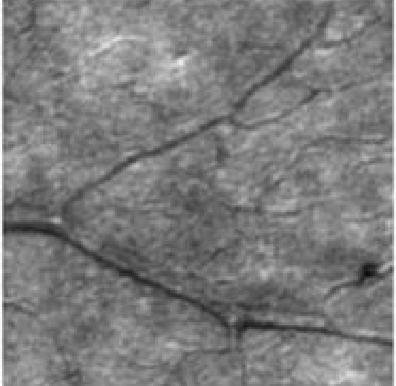
\includegraphics[width=0.75\textwidth, scale=0.75]{de_castro_channel_2.png}
		\caption{Image from \cite{castro_rapid_2016}, channel 2}
		\label{fig:de-castro-channel-b}
	\end{subfigure}
	\caption{The corresponding images of the same area in the retina captured by two imaging
		wavelengths for our own data \ref{fig:own-channel-a}\ref{fig:own-channel-b} and \ref{fig:de-castro-channel-a}\ref{fig:de-castro-channel-b}.
		It's obvious that the images from the two channels are not only temporally offset but
		spatially offset as well.
		This is because the imaging technique that is used to produce the time displacement between the channel also introduces some spatial offset which is known as seen in Fig \ref{fig:speed-of-cell-over-time}.
		The spatial offset is mostly constant and changes slowly as the video progresses and 
		can be easily fixed. 
	}
	\label{fig:corresponding-channels}
\end{figure}

In the same publication, a method for measuring the velocity of the erythrocytes is also described. %by using post-processing techniques.
The cells must be first detected.
By first normalizing the frames of the video for each channel and then applying a threshold to the images a binary image is created for each frame.
The threshold is N times the standard deviation of the pixel intensity over the all the frames of the video.
Then a morphological open operator is applied to the binary images to produce a set of location for the cells.
Instead of comparing the cell locations directly between the channels it is advised to create an ``average cell image'' by averaging all the cells for each frame.
By measuring the displacement of the ``average cell images'' between the two channels the average displacement and hence the velocity can be calculated\ref{fig:castro-average-cell}.

\begin{figure}[ht]
 	\centering
 	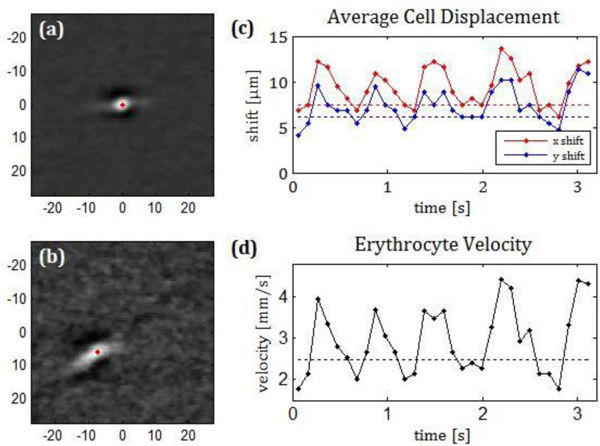
\includegraphics[width=0.5\textheight]{castro-average-cell.png}
 	\caption{Figure from \cite{castro_rapid_2016}.
 		In (a) we see the average cell created from the first channel and in
 		in (b) the corresponding average cell for the second channel that is 4.7 ms ahead
 		of the first .
 		By measuring the 
 		x and y displacement(c) the average red blood velocity(d) can be computed}.
 	 	We want to follow a similar process as shown in Fig \ref{fig:speed-of-cell-over-time}.
 	\label{fig:castro-average-cell}
\end{figure}

This method allows for measuring a bigger range of retinal capillary velocity than was previously possible as shown in the results from high frame rate fundus illumination system \cite{bedggood_direct_2012}, or on leukocytes using either the entoptic phenomenon \cite{riva_blue_1980}\cite{grunwald_effect_1993}, or other single channel imaging techniques with AOSLO \cite{martin_pulsatility_2009}\cite{martin_direct_2005}\cite{tam_speed_2011}\cite{tam_characterization_2011} as reported in \cite{castro_rapid_2016}.
The method in\cite{castro_rapid_2016} can measure velocities higher than was previously possible with the methods described before because red blood cells can be faster than white blood cells due to their size. 
It also produces comparable results to labeling with fluorescein\cite{yang_fluorescent_1997}\cite{paques_evaluation_2000} which is an invasive imaging method since it requires adding the artificial dye to the eye.
Additionally, this method is better for smaller vessels (capillaries)  while other techniques such as \cite{zhong_vivo_2008} or \cite{riva_laser_1972} are better for larger vessels.
One additional benefit of this method is that it allows for a bigger area of the retina to be image.
The benefit is twofold because we can  study a bigger retina area and also artifacts from eye movement can be corrected more easily using techniques such as \cite{dubra_registration_2010}.

Our team implement the same setup in \cite{castro_rapid_2016} but unfortunately the image processing pipeline to track the blood cells did not work for our case since, due to differences in the implementation, the cells from our setup lack the bright characteristic that was present in the cells in\cite{castro_rapid_2016}. 

\subsection*{Cell recognition and localization}
Consequently, we research other potential methods for identifying erythrocytes in our images.
In this light, we review the work done in image recognition and localization of conic photoeceptors in AOSLO images.
The conic shape and structure of the images of the phototoreceptors\ref{fig:bergelles-photoreceptors} is different from our images but since the rasters were generated using AOSLO techniques, they serve as good candidates for potentially similar implementations.

\begin{figure}[ht]
	\centering
	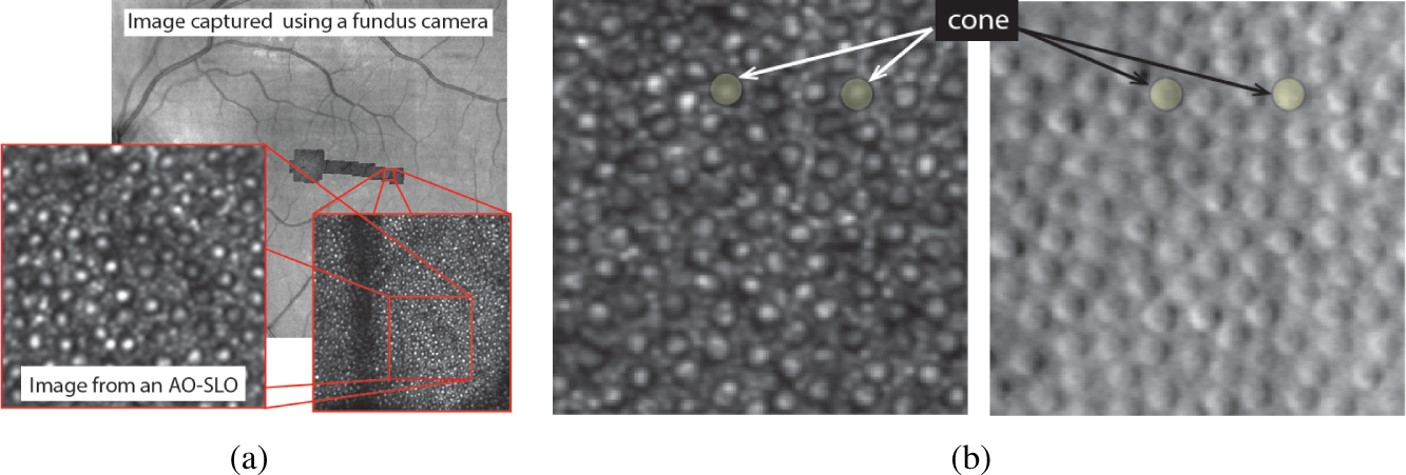
\includegraphics[width=\textwidth]{bergelles-photoreceptord.jpg}
	\caption{Figure of photoreceptors mosaic from \cite{bergeles_unsupervised_2017}.
		In (b) we see images captured with two different AOSLO techniques.
	}
	\label{fig:bergelles-photoreceptors}
\end{figure}
 
The publication presents a way to classify the conic photoreceptors using an image processing pipeline that uses SVN.
In brief, the pipeline includes the photoreceptor's size estimation using an automated process (Yellott's ring\cite{cunefare_automatic_2016} \cite{cooper_automatic_2013}) by setting it manually, use of bilateral and a Gaussian filter, adaptive histogram equalization, adaptive sliding-window enhancement that is applied to enchance the contrast between the left/dark and right/bright sides of the cones, aggressive thresholding to create a binary image, non-overlapping extremal region detection to detect the centroids, a preliminary model for cone extraction and finally a model for refinement and cone detection using a Support Vector Machine (SVM). 
The process is described with great detail in the paper.
There are 11 configurable hyperparameters.
The results reported in the paper show that the model is precise and it's results are comparable to a human grader for images of healthy retinas and have a positive precision and recall on images of retinas with Stargardt disease.
It's also reported that the model can outperform the, at the time, state of the art model developed in\cite{cunefare_automatic_2016}.

Although the model shows promising results, it might not be the best choice for erythrocyte detection in our images. 
The method creates a cone-model that accounts for the characteristic shape and intensity of the photoreceptor cells.
In addition, the model is dependent on the spatial arrangement of the photoreceptor mosaic. 
As a result, when the model is presented with images of the photoreceptor mosaic of people with Stargard disease, which is more sparse, it's performance drops and both the precision and recall of the model are significantly lower.
For this reason, the parameter configurations and control will most likely not work for our problem, since our erythrocyte images not only have a different shape, they also have a different structure.

Hence, it was decided to follow a different paradigm.
Deep learning was shown to outperform traditional machine learning techniques for 
a lot of imaging tasks including image classification.
Deep networks learn features directly from the data and do not rely to ad-hoc rules
that are unique to the data-set.
As a result, such networks are more adaptable.
This is more appealing for our case because deep learning models can be
generic and a model that is a trained for a particular dataset can be
adapted  to be used for other datasets.
One drawback of deep learning is that it can be outperformed from traditional machine learning techniques when the the amount of training data is little.
This can be circumvented with techniques such as data augmentation\cite{perez_effectiveness_2017} which was shown to work with great success in the past\cite{ronneberger_u-net_2015}.
Deep Convolution Neural Networks (CNNs) have been shown to work for different image analysis tasks in many fields including optical imaging\cite{gulshan_development_2016, perez_effectiveness_2017, li_cross-modality_2016, fu_retinal_2016, fang} with great performance.

For this reason we would like to review the method described \cite{cunefare_open_2017} and mention \cite{cunefare_deep_2018}.
Both of this methods try to classify and locate conic photoreceptors in
AOSLO images using image classification deep neural networks.
We believe this work can be adapted for our use-case as well since
the implementation for cell detection and localization is not dependent on the structure and appearance of the cone cells.
Next, we would summarize the implementation that is described in the paper.
First, images of the photoreceptor mosaic are captured and experts mark the centers of each cone.
To create a training set for the binary classifier we need images for cone and non-cone cells.
A window of a fixed size is drawn around the marked centers to extract patches of cones.
To produce images of negatives a voronoi pattern is created around the centers.
Then random points from the edges of the voronoi pattern are selected as centers for the non-cone patches.
This process is demonstrated in Fig\ref{fig:cunefare-training-data-generation}.

\begin{figure}[h]
	\centering
	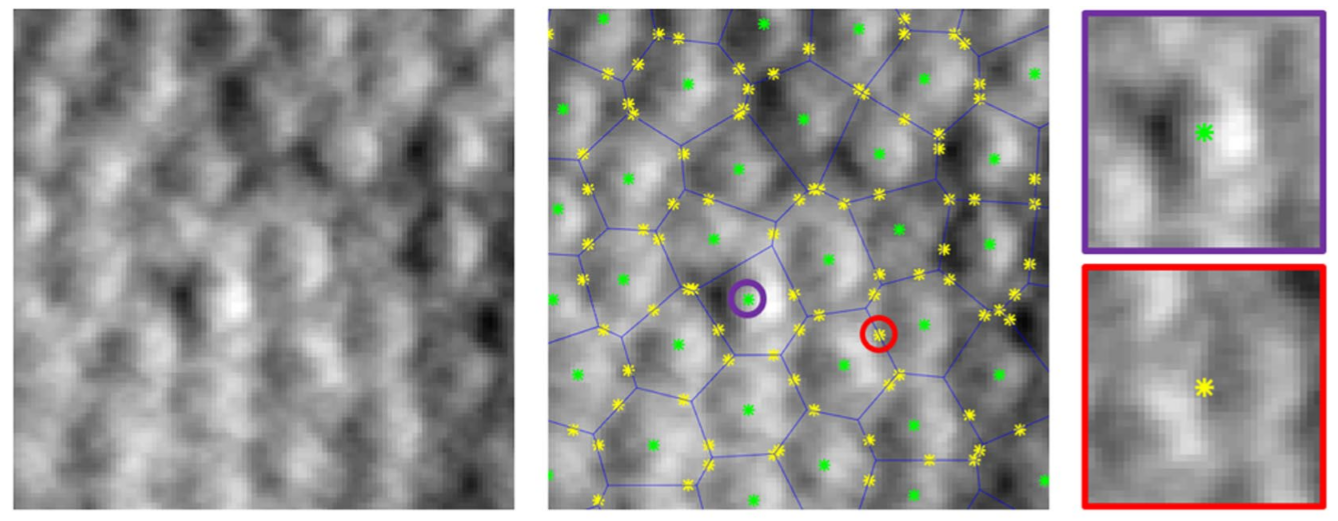
\includegraphics[width=\textwidth]{cunefare_generating_data.png}
	\caption{Image from \cite{cunefare_open_2017}. Training data generation process for the CNN training. \textbf{(a)} The original image of the 
	photoreceptor mosaic, \textbf{(b)} Image (a) with the center of the photoreceptors marked by an expert and a voronoi diagram around them. Points on the voronoi edges are randomly selected as centers of non-photoreceptor patches. 
    \textbf{(c)} An example of a cone (top) and non-cone (bottom) patch extracted from the marked image (b).}
	\label{fig:cunefare-training-data-generation}
\end{figure}


Once the training set is created the CNN classifier can be trained to detect cone from non-cone images.
The CNN described in\cite{cunefare_open_2017} is a modification of the famous AlexNet\cite{krizhevsky_imagenet_2012}.
It consists of Convolutional layers to generate feature maps, pooling layers which are known to improve computational performance and increase invariance to small distortions\cite{jarrett_what_2009},
Rectified linear units (ReLU) activation layers to introduce non-linearities\cite{jarrett_what_2009},
batch normalization layers which are reported to increase training speed and reduce overfitting by normalizing layer inputs using their mean statistic\cite{ioffe_batch_2015}.
In the end there are fully connected  layers, again with ReLU activations, for the final classification part.
The last fully connected layer has two outputs and is fed to a soft-max layer that turns the output to probability distribution for cone and non-cone\cite{bishop_pattern_recognition_2006}.
For the training process the weights are randomly initialized. 
Each iteration, also called an epoch, a subset of the training set, called a mini-batch, is fed to the network.
For each image in the mini-batch a label is predicted with a probability distribution from the soft-max layer, i.e 75 per cent cone and 25 per cent non-cone.
In the training process, because the label is known for each image, 
a loss function measures the distance of the predicted output and the actual label.

Proportionally to this distance, the network adjusts the weights, with a process called back propagation.
This whole training process is called gradient descent because during the forward pass a gradient is calculated for each weight with the goal to minimize the training loss.

With sufficient training data the network can potentially classify cones from non-cones with a high accuracy.
We should mention that, part of the dataset should be used just for testing the performance of the classifier and should not be used for training.
The photoreceptors must then be localized in the image.
In \cite{cunefare_open_2017}, a patch is created around every pixel of the image and all the patches are classified with the trained CNN.
The result is a gray-scale image with a probability of each pixel being the center of a cone.
Next, a Gaussian smoothing is applied on the probability map followed by an extended-maxima transform.
The resulting binary image is thresholded.
Finally, the center of the remaining clusters is considered to be the center of the cone.
For additional information for the hyperparameter values please see \cite{cunefare_open_2017}.

The results are compared against the gold standard for detecting photoreceptors that uses graph theory and dynamic programming (GTDP)\todo{cite} and a previous work
that we mentioned earlier that uses adaptive filtering and local detection (AFLD) \cite{cunefare_automatic_2016}.
In both cases the  results are very comparable with a true positive rate ranging from 0.943 to 0.989 and a false discovery rate of 0.034 and as low as 0.003.
For a more detailed description of the evaluation method please refer to\cite{cunefare_open_2017}.

The results are very appealing since it shows that the model can compete with state of the art methods.
Contrary to the other techniques, it has the advantage that it can be adapted for applications with different modalities since it uses a modified generic CIFAR network.
The GTDP and AFLD models were created with assumptions and rules that are specific for the photoreceptor mosaic.
The software for the  model in\cite{cunefare_automatic_2016} is open source and is shared by the authors.
Furthermore, they encourage the use of software for testing and adaption to new training data sets and imaging conditions.

Image classification using CNNs can potentially solve the problem of locating the red blood cells in our videos.
Once the red blood cells are located correspondence must be made between the two channels of the frame to measure the velocity.
An alternative is to use the method used in\cite{castro_rapid_2016} with the calculation 
of the ``average cell"\ref{fig:castro-average-cell}.
Because this method creates ``average cell" for the two channels by adding all the detected
cells it is required for the cells to move in the same direction. 
For example, if we take the mean of two erythrocytes that move in opposite directions then their ``average cell" image will be in the same position and the speed would be 0.
The solution in\cite{castro_rapid_2016} is to manually select a small capillary segment.
This could be also implemented for our case since in a single video from a patient 
the capillary structure is guaranteed to stay the same.
Since a fully automatic tool is desired, it is useful
to research on existing methods for blood vessel segmentation.
\subsection*{Capillary segmentation}
By having a capillary segmentation the benefit is threefold,
The search-space for potential blood cells would be drastically reduced since
most of the image consists of non-cells making the localization of the cells more efficient.
In addition, the training set should contain more meaningful non-cell images than simply empty patches, increasing the performance of the classifier and potentially reducing false positives.
Finally, if the capillary segmentation is known then we could analyze a
small segment of it at a time so that it's guaranteed that the blood cells move 
in the same direction.

Currently, there is a growing literature for blood vessel segmentation 
in retinal images\cite{liskowski_segmenting_2016}\cite{fu_retinal_2016}\cite{li_cross-modality_2016}. 
However, the data-set for this problems focuses on fundus imaging\cite{fraz_blood_2012} and is focused on bigger blood vessels in the 
retina (arteries and veins) and not on capillaries. 
Additionally, fundus imaging is very different and produces images with very different features than the ones we have.
As previously stated, we could potentially adapt existing deep learning techniques for our use-case.
One promising such segmentation network is DeepVessel\cite{fu_deepvessel_2016} which produces state of the art results.
To train for segmentation using a supervised machine learning method it is required to have a ground truth for the capillaries which we currently don't
have.
We could produce ground truth  for some of our images but the amount of data could not be sufficient to train a network.
Data augmentation techniques could be used to decrease the amount of data needed.
Moreover, transfer learning is shown to work\cite{jiang_retinal_2018} when 
there is a lack of labeled data available.
With transfer learning, we could potentially train a neural network like
DeepVessel with publicly available fundus images and then retrain part of 
the network with images from our training data.


\section{Proposed Method} 
In this section we propose a method that takes inspiration from methods that were previously described.

The end-goal of this dissertation is to create a tool that takes a video of the retina
captured with AOSLO and produces statistics about the velocity of the blood flow 
based on tracking the erythrocytes moving in the capillaries.
As mentioned before, the method for capturing the images is the same as in\cite{castro_rapid_2016}.
Ideally, we would like the process to be automatic but in case not all components
of the system are implemented due to time constraints the user should be able
to mark areas with capillaries.

The process of tracking and measuring the blood cells can be broken down to three 
big steps.
First the locations of the blood cells must be located in both channels for each frame of the video.
Next, the correspondence between the cells must be established.
Finally, since we know the time disparity between the two channels we can measure the average velocity of the blood flow\ref{fig:speed-of-cell-over-time}.

\begin{figure}[ht]
	\centering
	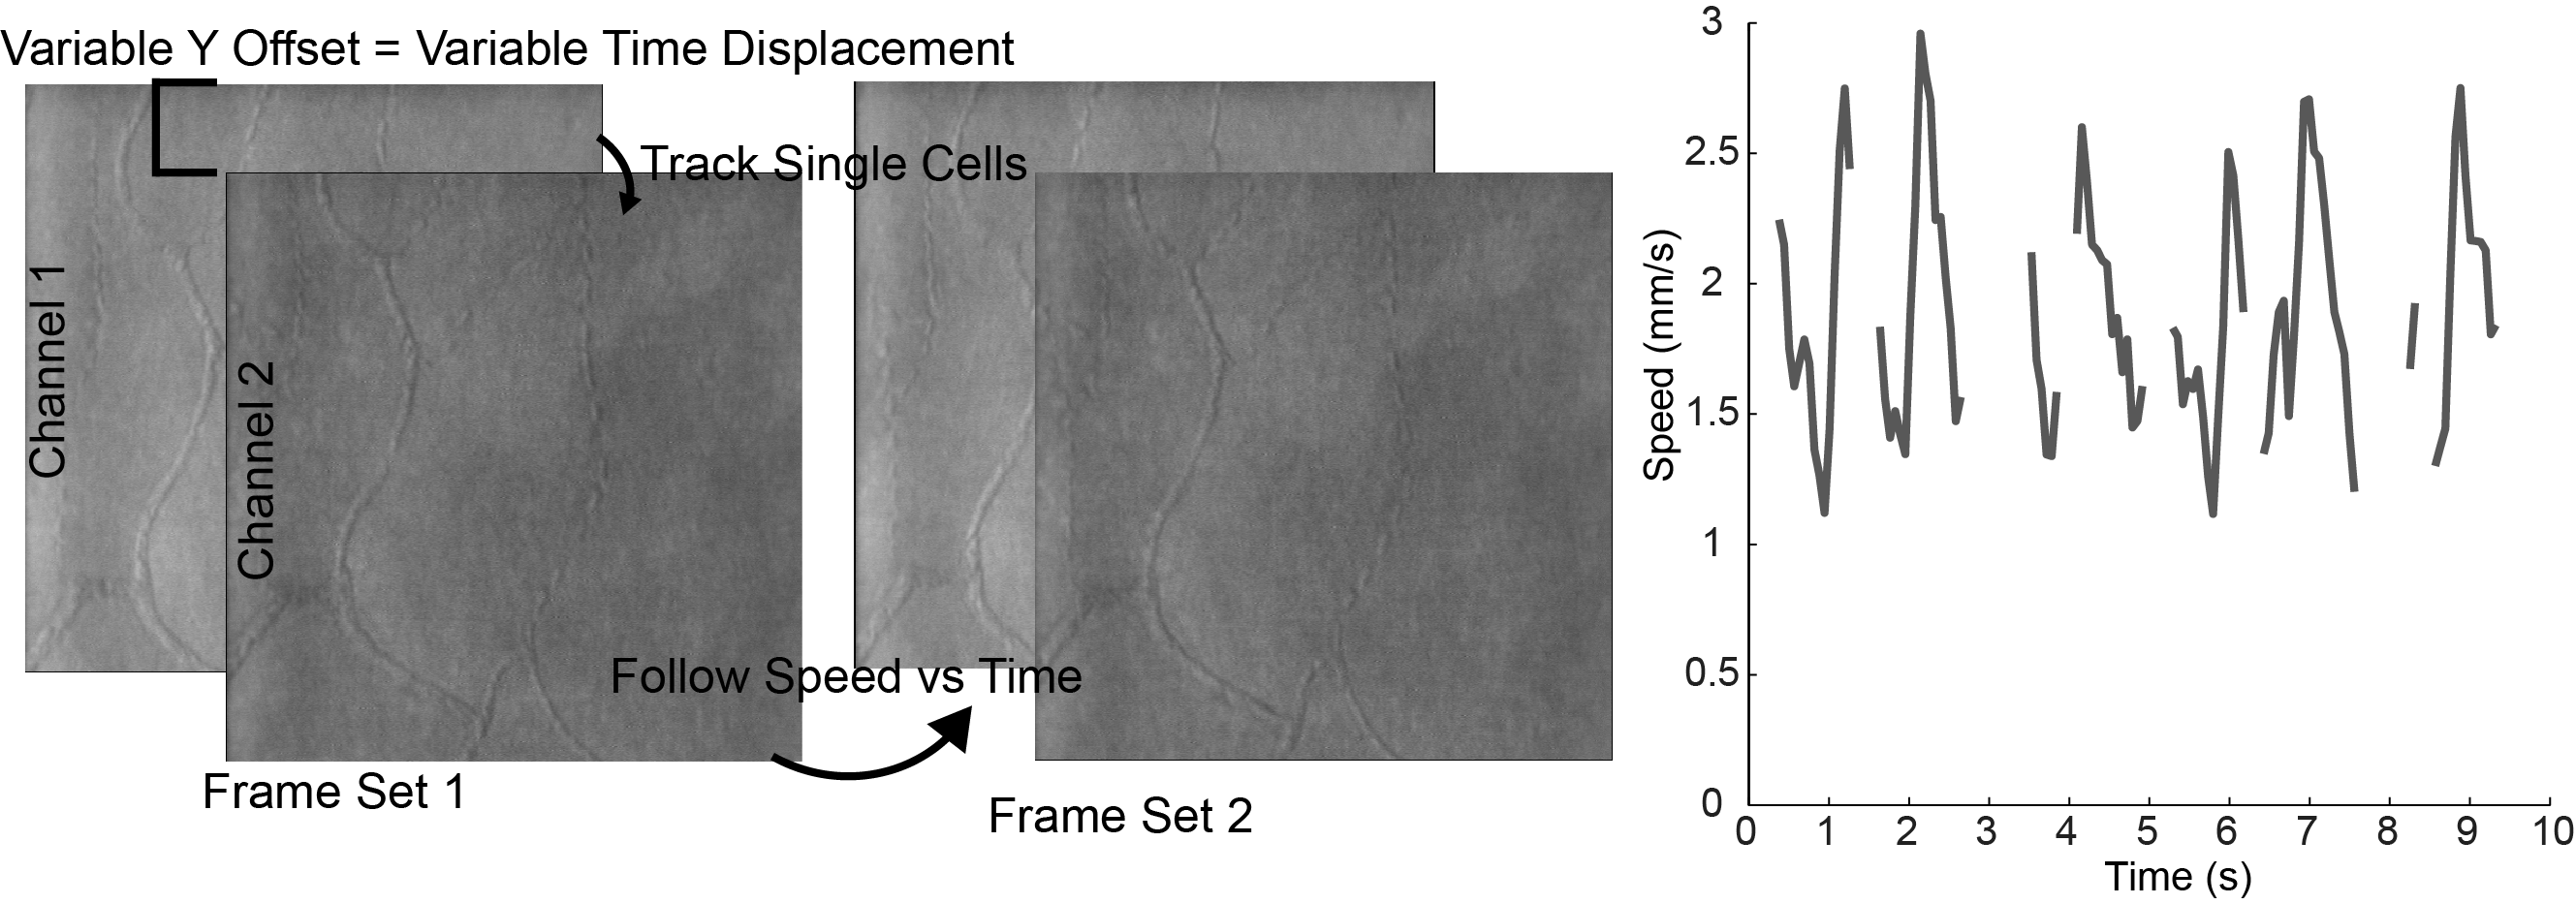
\includegraphics[width=\textwidth]{spatial_offset.png}
	\caption{Measuring the speed of a red blood cell over time.}
	\label{fig:speed-of-cell-over-time}
\end{figure}

For the first part, we decided to follow the work done in \cite{cunefare_open_2017}.
The process to localize the erythrocytes will be similar to what was described 
in the previous section.
In brief, the training set for the cell and no-cell images should be created by 
extracting a fixed window patches around cell and no-cell locations\ref{fig:own-data-blood-cells}.
The cell locations are marked by an expert and the no-cell
locations are extracted from the voronoi pattern with the method described
in\cite{cunefare_open_2017}.

\begin{figure}[ht]
	\centering
	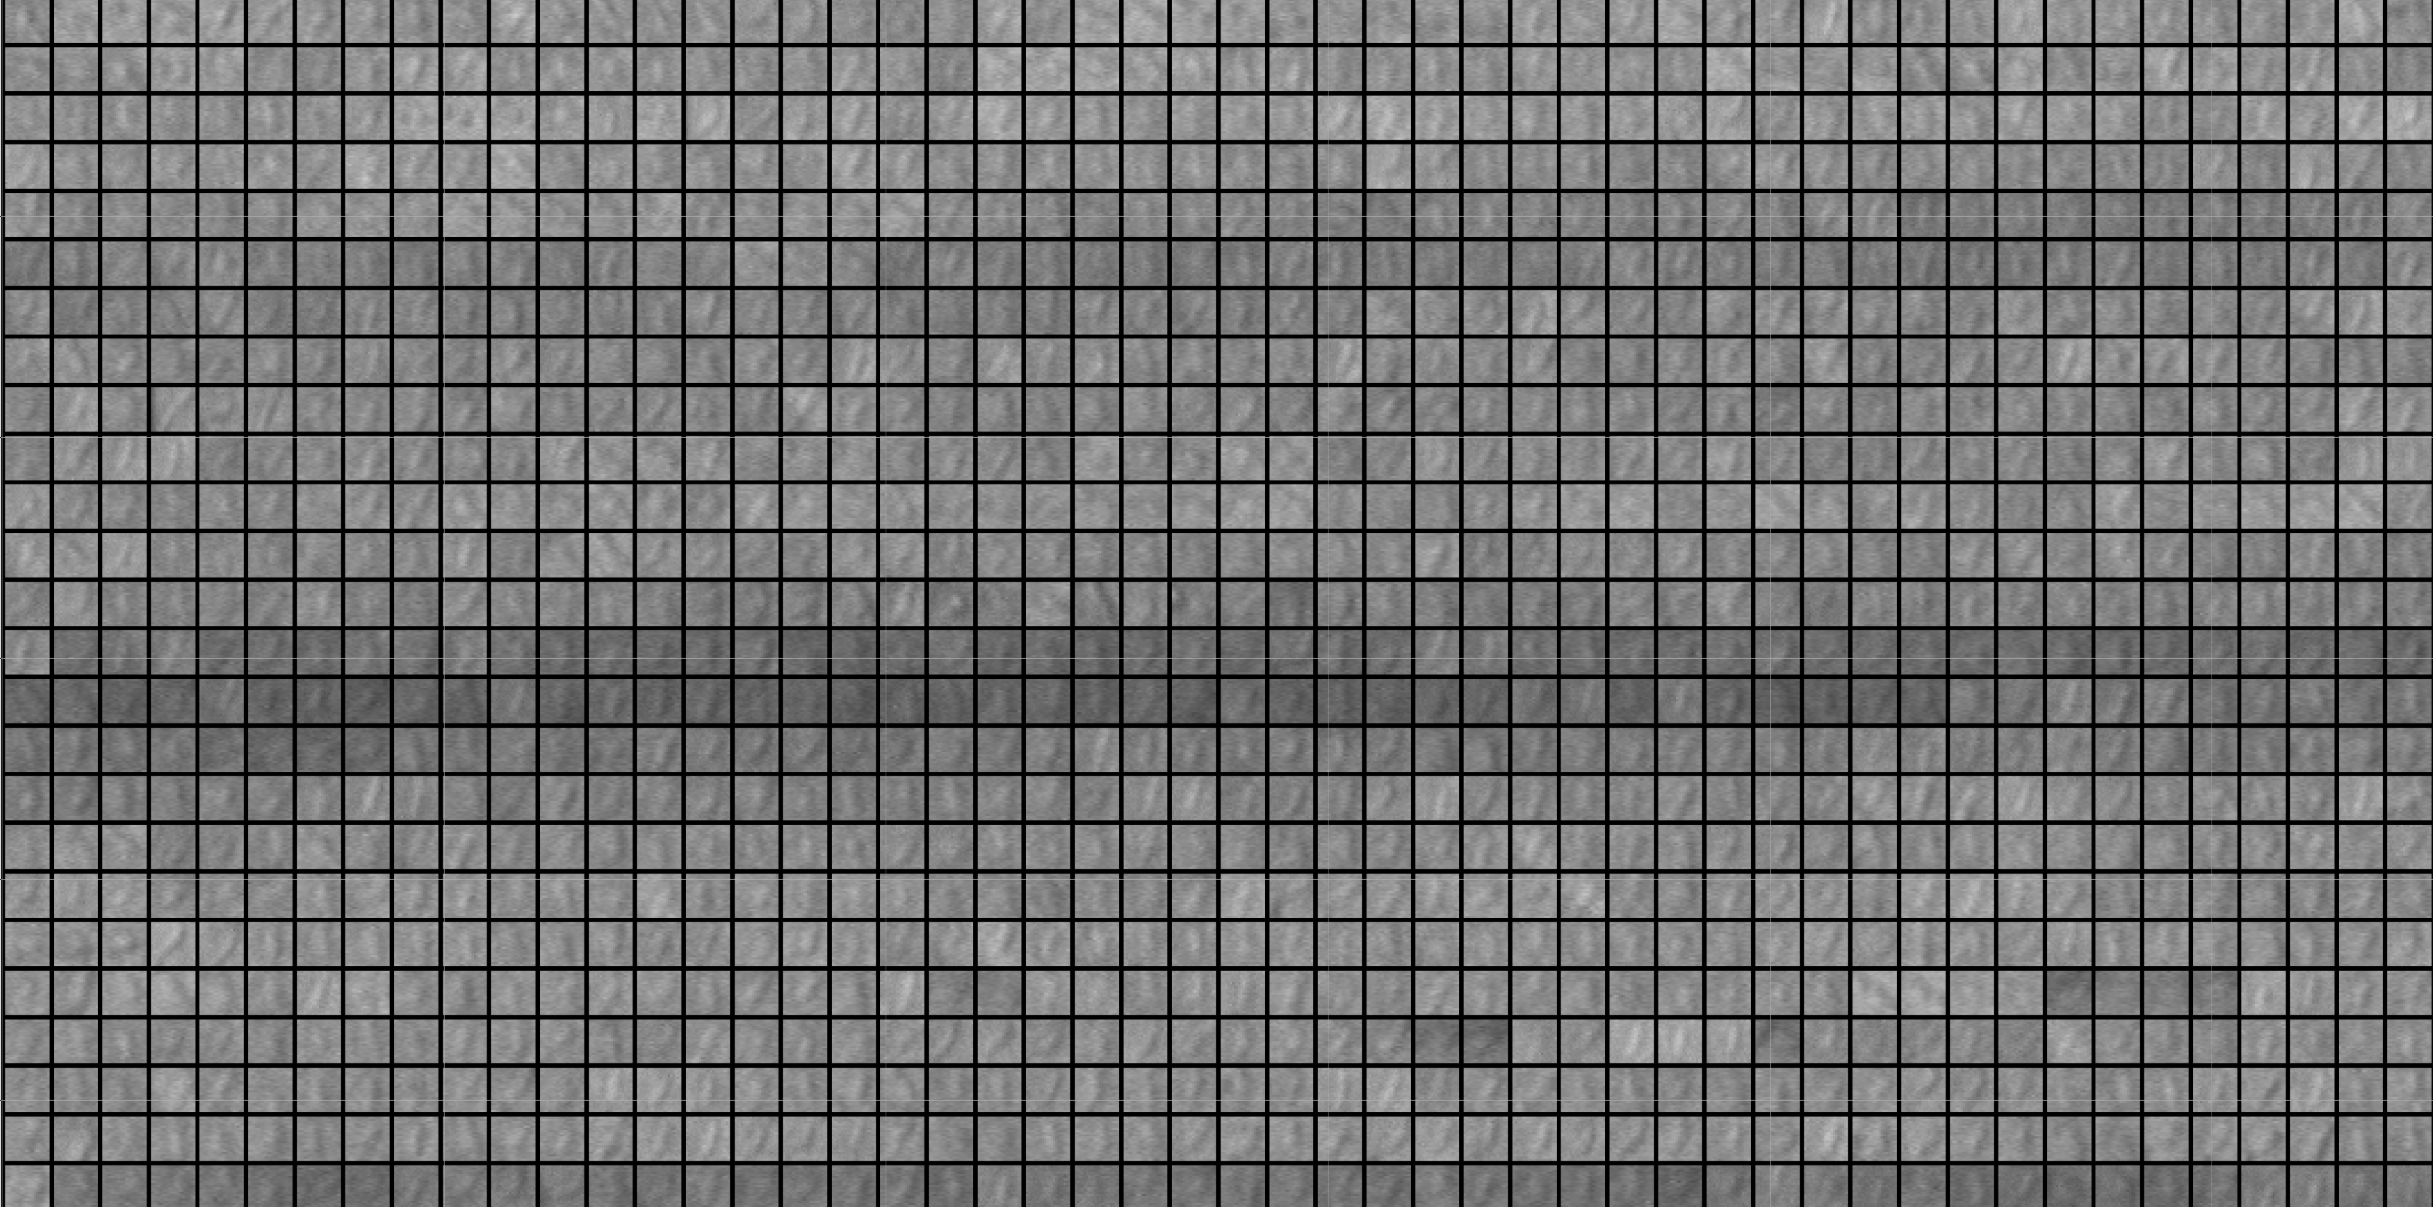
\includegraphics[width=\textwidth]{extracting_data_own.png}
	\caption{Red blood cell patches extracted from \href{https://youtu.be/-7ew5sqOaTo}{(media)}. }
	\label{fig:own-data-blood-cells}
\end{figure}

Then a AlexNet\cite{krizhevsky_imagenet_2012}-like CNN should be trained until the desired performance is achieved.
A potential challenge for this stage would be the lack of sufficient data quantity.
To circumvent this data augmentation could be used.
The red blood cell patches seem to have similar size and intensities so we believe that it could possible to augment our data-set with fake images by transforming existing ones.
Another likely problem that could arise is overfitting to the training data.
Because the retina of different subjects can have different reflective properties, and the conditions of the recording session are also different from
person to person it's very likely that the network will fail when presented with
new and unseen images that are dissimilar to the the training data.
To get around this problem, regularization techniques can be applied such as dropout layers, early stopping, L2 \& L1 regularization\cite{Goodfellow-et-al-2016} or, again, with data augmentation\cite{Goodfellow-et-al-2016} . 

Assuming a classifier with good performance is achieved, the next step is to 
locate the cells.
Firstly, a patch should be extracted around every pixel. Each patch should be 
fed through the classifier.
Just like in \cite{cunefare_open_2017} the resulting probability map should be then be smoothed and extended-maxima transform must be applied.
After weak candidates should be filtered.
The centers of the remaining clusters is the predicted location of the cells.

For the next step, instead of directly establishing correspondence,
it was decided the ``average cell" technique from\cite{castro_rapid_2016}
should be implemented.
The cells for each channel should be added and then averaged.
The displacement of the average cell shows the average displacement 
and can be used to calculate the average velocity.
As previously mentioned, the blood cells should move in the same direction in the segment of the capillary or else the estimated velocity is wrong\ref{fig:segment-fail-example}.

\begin{figure}[ht]
	\centering
	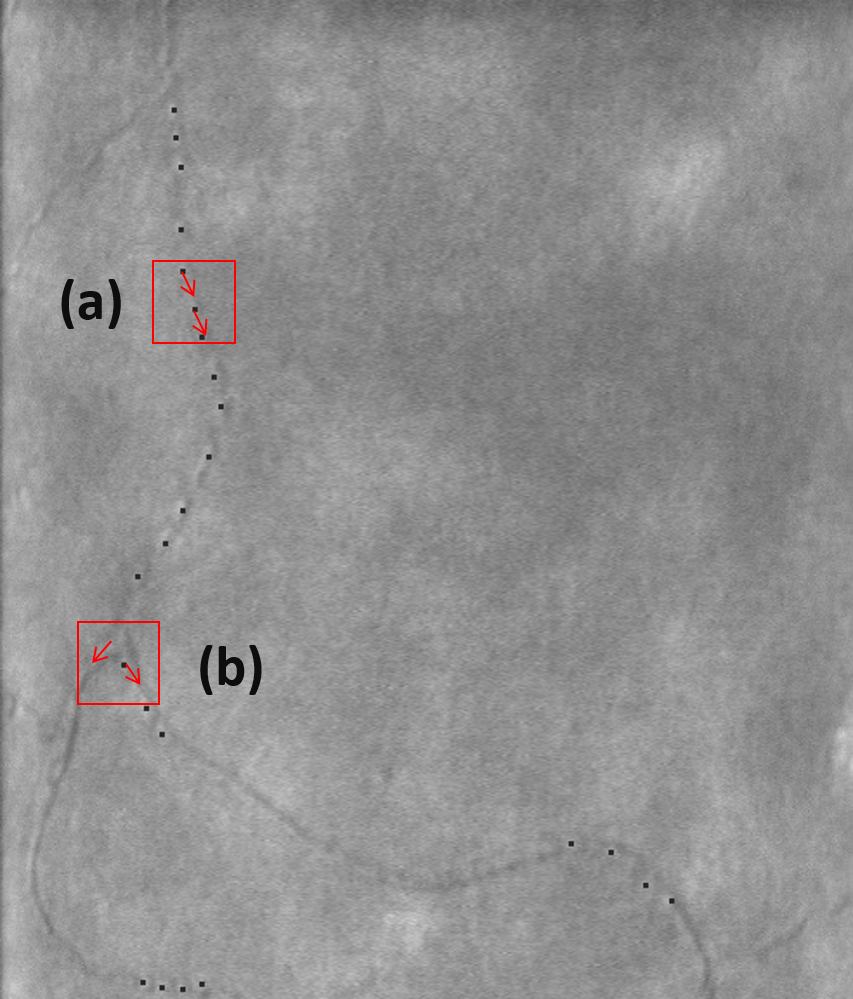
\includegraphics[width=0.5\textwidth, scale=0.5 ]
	{segment-example.png}
	\caption{An example where ``average cell" can produce wrong results. In segment (a) the cells move in the same direction and the average displacement can be calculated correctly.
	In (b), because the cells move in different directions, the velocity will not be correct.}
	\label{fig:segment-fail-example}
\end{figure}
For this part, the capillary segment can be manually selected by the user. 
Alternatively, assuming capillary segmentation is achieved we can create small segments all over the capillary and create an average 
cell for each segment.
Finally, the corresponding velocity magnitude for each segment could then be summed up to get the average velocity of the blood cells for that frame.

As a final goal, we would like to aggregate this work into a functional
tool that could be used to easily measure the patients blood flow.

\section{Proposed Evaluation}

The performance of the model could be evaluated in two steps.
One for the classifier and how correctly will it be able to locate 
the erythrocytes and one for the correctness of the velocity measurement.

For the first part, we could follow the validation method used in\cite{cunefare_open_2017}.
In brief we could count cells as correctly located (true positive) when their predicted location is in close proximity to the experts marking.
If the predicted location is further than a certain range from the experts marking then it should be considered wrong (false positive).
The number of marked $N_{\text{model}}$ blood cells is the sum of the true positives and false positives.
The number of cells marked by the expert $N_{\text{expert}}$ is the sum of the true positives $N_{TP}$ and the false negatives $N_{FN}$.
We can measure true positive rate, false discovery rate and Dice’s coefficient\cite{dice_measures_1945}:
\[
\text{True Positive Rate} =  \frac{N_{TP}}{N_{\text{expert}}}
\] 
\[
\text{False discovery Rate} = \frac{N_{FP}}{N_{\text{model}}}
\] 
\[
 \text{Dice's coefficient} = \frac{2N_{TP}}{(N_{\text{expert}}+ N{\text{model}})}
\]
In an ideal world, true positive rate and  Dice's coefficient  should be 1 while false discovery rate should be 0.

The correct estimation of the velocity is directly related to the performance of the classifier.
We could measure error 


\end{document}
